
\documentclass[aspectratio=169,xcolor=dvipsnames]{beamer}
%\usetheme{SimplePlus}

\usepackage{hyperref}
\usepackage{graphicx} % Allows including images
\usepackage{booktabs} % Allows the use of \toprule, \midrule and \bottomrule in tables

%----------------------------------------------------------------------------------------
%	TITLE PAGE
%----------------------------------------------------------------------------------------

\title[RegMet]{Reguleringsmetoder} % The short title appears at the bottom of every slide, the full title is only on the title page
%\subtitle{Subtitle}

\author[Fred-Olav] {Fred-Olav Mosdal}

\institute[Gand VGS] % Your institution as it will appear on the bottom of every slide, may be shorthand to save space
{
    Gand VGS \\
    VG3 Automasjon
}
\date{\today} % Date, can be changed to a custom date


%----------------------------------------------------------------------------------------
%	PRESENTATION SLIDES
%----------------------------------------------------------------------------------------

\begin{document}
%\section{Cascade control}
%
%A simple control system drawn in block diagram form looks like this:
%
\begin{frame}
\titlepage
\end{frame}
%$$\includegraphics{cont05.eps}$$
%
%Information from the measuring device (e.g. transmitter) goes to the controller, then to the final control device (e.g. control valve), influencing the process which is sensed again by the measuring device.  The controller's task is to inject the proper amount of negative feedback such that the process variable stabilizes over time.  This flow of information is collectively referred to as a feedback control \textit{loop}.  \index{Negative feedback}
%
%To \textit{cascade} controllers means to connect the output signal of one controller to the setpoint of another controller, with each controller sensing a different aspect of the same process.  The first controller (called the \textit{primary}, or \textit{master}) essentially ``gives orders'' to the second controller (called the \textit{secondary} or \textit{slave}) via a \textit{remote setpoint} signal.  \index{Cascade control strategy}  \index{Remote setpoint}  \index{Setpoint, remote}
%
%\filbreak
%
%Thus, a cascade control system consists of two feedback control loops, one nested inside the other:  
%
\begin{frame}
	\frametitle{Kaskaderegulering}
	Med kaskaderegulering ønsker en å oppnå større stabilitet på den primære prosessvariablen, ved å regulere en sekundær prosessvariabel alt etter behovene til den primære. Et absolutt krav for at kaskaderegulering skal virke er at den sekunære variabelen har kortere tidskonstant. (ca 3-4 ganger kortere)
	$$\includegraphics[height=6cm]{cont14.eps}$$
\end{frame}
%$$\includegraphics{cont14.eps}$$
%
%A very common example of cascade control is a \textit{valve positioner}, which receives a command signal from a regular process controller, and in turn works to ensure the valve stem position precisely matches that command signal.  The control valve's stem position is the process variable (PV) for the positioner, just as the command signal is the positioner's setpoint (SP).  Valve positioners therefore act as ``slave'' controllers to ``master'' process controllers controlling pressure, temperature, flow, or some other process variable.
%
%The purpose of cascade control is to achieve greater stability of the primary process variable by regulating a secondary process variable in accordance with the needs of the first.  An essential requirement of cascaded control is that the secondary process variable be faster-responding (i.e. shorter lag and dead times) than the primary process variable. 
%
%An analogy for understanding cascade control is that of \textit{delegation} in a work environment.  If a supervisor delegates some task to a subordinate, and that subordinate performs the task without further need of guidance or assistance from the supervisor, the supervisor's job is made easier.  The subordinate takes care of all the little details that would otherwise burden the supervisor if the supervisor had no one to delegate to.  This analogy also makes it clear why the secondary process variable must be faster-responding than the primary process variable: the supervisor-subordinate management structure fails to work if the supervisor does not maintain focus on long-term goals (i.e. longer-term than the completion time of the tasks given to subordinates).  If a supervisor focuses on achieving goals that are shorter-term than the time required for subordinates to complete their assignments, the supervisor will inevitably call for ``course changes'' that are too quick for the subordinates to execute.  This will lead to the subordinates ``lagging'' behind the supervisor's orders, to the detriment of everyone's satisfaction.
%
%\vskip 10pt
%
%\filbreak
%
%An example of cascade control applied to a real industrial process is shown here, for a \textit{dryer} system where heated air is used to evaporate water from a granular solid.  The primary process variable is the outlet air exiting the dryer, which should be maintained at a high enough temperature to ensure water will not remain in the upper layers of the solid material.  This outlet temperature is fairly slow to react, as the solid material mass creates a large lag time:
%
%$$\includegraphics{cont16.eps}$$
\begin{frame}
	\frametitle{Eksempel på prosess med behov for kaskaderegulering}

	$$\includegraphics[height=7cm]{cont16.eps}$$
\end{frame}

%
%There are several parameters influencing the temperature of the outlet air other than the moisture content of the drying material.  These include air flow, ambient air temperature, and variations in steam temperature.  Each one of these variables is a \textit{load} on the process variable we are trying to control (outlet air temperature).  If any of these parameters were to suddenly change, the effect would be slow to register at the outlet temperature even though there would be immediate impact at the bottom of the dryer where the heated air enters.  Correspondingly, the control system would be slow to correct for any of these changing loads.
%
%\filbreak
%
%We may better compensate for these loads by installing a second temperature transmitter at the inlet duct of the dryer, with its own controller to adjust steam flow at the command of the primary controller:
%
\begin{frame}
	\frametitle{Eksempel på prosess med kaskaderegulering}

	$$\includegraphics[height=7cm]{cont15.eps}$$
\end{frame}
%$$\includegraphics{cont15.eps}$$
%
%Now, if any of the loads related to incoming air flow or temperature vary, the secondary controller (TC-1b) will \textit{immediately} sense the change in dryer inlet temperature and compensate by adjusting steam flow through the heat exchanger.  Thus, the ``slave'' control loop (1b) helps stabilize the ``master'' control loop (1a) by reacting to load changes long before any effect might manifest at the dryer outlet.
%
%A helpful way to think of this is to consider the slave controller as \textit{shielding} the master controller from the loads previously mentioned (incoming air flow, ambient temperature, and steam temperature).  Of course, these variables still act as loads to the slave controller, as it must continuously adjust the steam valve to compensate for changes in air flow, ambient air temperature, and steam temperature.  However, so long as the slave controller does a good job of stabilizing the air temperature entering the dryer, the master controller will never ``see'' the effects of those load changes.  Responsibility for incoming air temperature has been delegated to the slave controller, and as a result the master controller is conveniently isolated from the loads impacting that loop.
%
%To re-emphasize an important point, one of the non-negotiable requirements for cascade control is that the secondary (slave) loop must be \textit{faster-responding} than the primary (master) loop.  Cascade control cannot function if this speed relationship is reversed.  Temperature controller TC-1b is able to be a slave to controller TC-1a because the natural response time of the temperature at the dryer's bottom is much shorter than at the dryer's top with respect to any changes in steam valve position.
%
%\vskip 10pt
%
%\filbreak
%
%A common implementation of cascade control is where a flow controller receives a setpoint from some other process controller (pressure, temperature, level, analytical, etc.), fluid flow being one of the fastest-responding process types in existence.  A feedwater control system for a steam boiler -- shown here in pneumatic form -- is a good example: 
%
%$$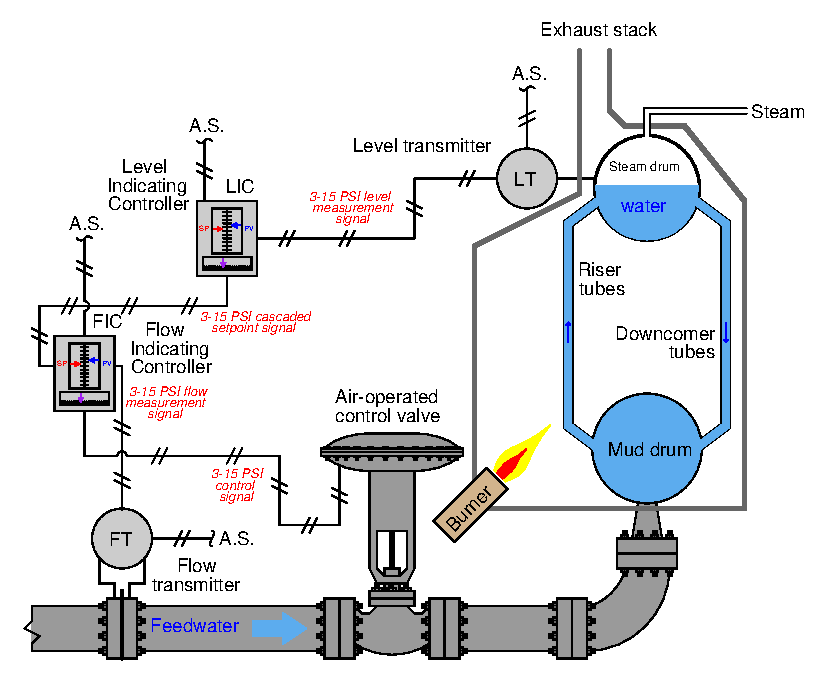
\includegraphics{cont19.eps}$\begin{frame}
	\begin{frame}

	\frametitle{Eksempel på prosess med kaskaderegulering}

	$$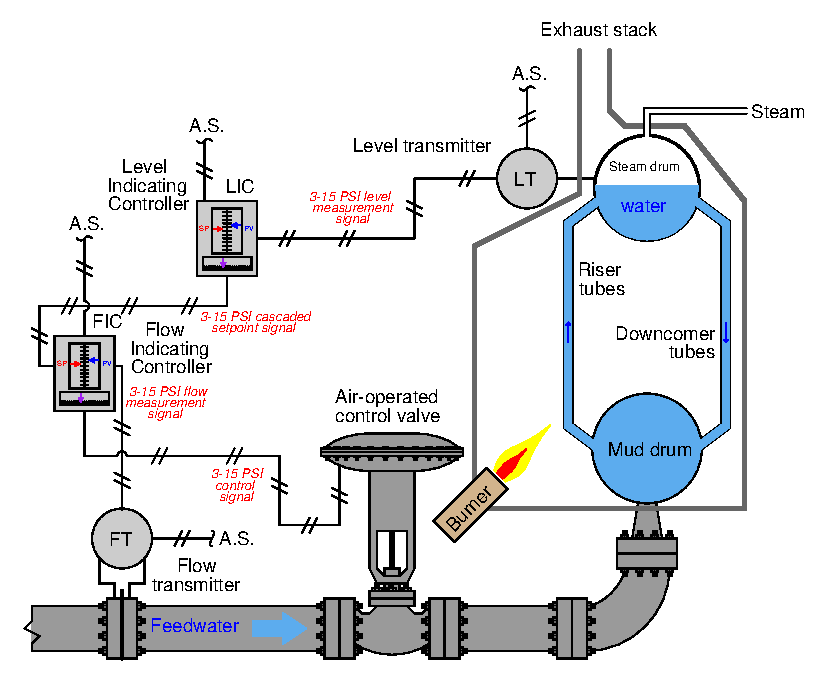
\includegraphics[height=7cm]{cont19.eps}$$
\end{frame}
%
%The ``secondary'' or ``slave'' flow controller works to maintain feedwater flow to the boiler at whatever flow rate is desired by the level controller.  If feedwater pressure happens to increase or decrease, any resulting changes in flow will be quickly countered by the flow controller without the level controller having to react to a consequent upset in steam drum water level.  Thus, cascade control works to guard against steam drum level instability resulting from changes in the feedwater flow caused by factors outside the boiler.  As stated previously, the slave (flow) controller effectively \textit{shields} the master (level) controller from loads in the feedwater supply system, so that master controller doesn't have to deal with those loads.
%
%This level/flow cascade control system also embodies the principle of the secondary (slave) loop being faster-responding than the primary (master) loop.  Water flow is an inherently fast process, the flow rate responding immediately to changes in valve position.  By contrast, water level is a much slower-responding type of process.  If you perform a ``thought experiment'' where the feedwater valve is suddenly opened fully, it is easy to see that the feedwater flow rate will immediately reach its full (100\%) value while the steam drum's water level will merely begin to rise, taking time to reach its full (100\%) value.
%
%\filbreak
%
%It is worth noting that the inclusion of a flow control ``slave'' loop to this boiler water level control system also helps to overcome a potential problem of the control valve: nonlinear behavior.  In the control valves chapter, we explore the phenomenon of \textit{installed valve characteristics} (Section \ref{installed_valve_characteristic} beginning on page \pageref{installed_valve_characteristic}), specifically noting how changes in pressure drop across a control valve influences its throttling behavior.  The result of these pressure changes is a non-linearization of valve response, such that the valve tends to be more responsive near its closed position and less responsive near its open position.  One of the benefits of cascaded flow control is that this problem becomes confined to the secondary (flow control) loop, and is effectively removed from the primary control loop.  To phrase it simply, distorted valve response becomes ``the flow controller's problem'' rather than something the level controller must manage.  The result is a level control system with more predictable response.  \index{Installed valve characteristic} 
%
%\vskip 10pt
%
%\filbreak
%
%A classic example of cascade control strategy is found in \textit{motion control} applications, where an electric motor is used as the final control element to precisely position a piece of machinery.  In this capacity, the motor is usually called a \textit{servo}.  Robotic systems make extensive use of servo motors and cascaded control loops to modulate power to those motors.  The following illustration shows a triple-cascade control system\footnote{Interestingly, servo motor control is one application where \textit{analog} loop controllers have historically been favored over digital loop controllers, simply for their superior speed.  An opamp-based P, PI, or PID controller is lightning-fast because it has no need to digitize any analog process variables (analog-to-digital conversion) nor does it require time for a clock to sequence step-by-step through a written program as a microprocessor does.  Servomechanism processes are inherently fast-responding, and so the controller(s) used to control servos must be faster yet.} for a motor-actuated elevator, precisely controlling the position of the elevator through cascaded velocity and motor current control:  \index{Motion control system}  \index{Triple-cascaded loops}  \index{Servo motor control}
%
%$$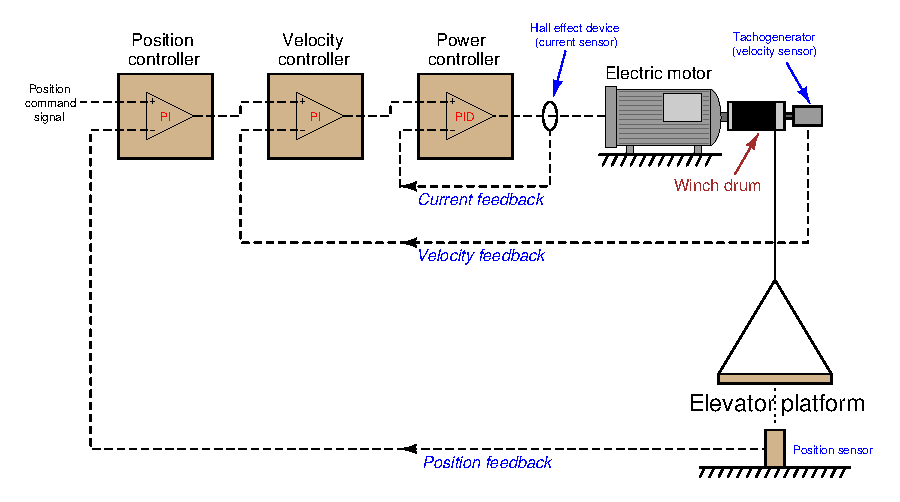
\includegraphics{cont75.eps}$$
	\begin{frame}
		\frametitle{Servosystem med kaskaderegulering}

		$$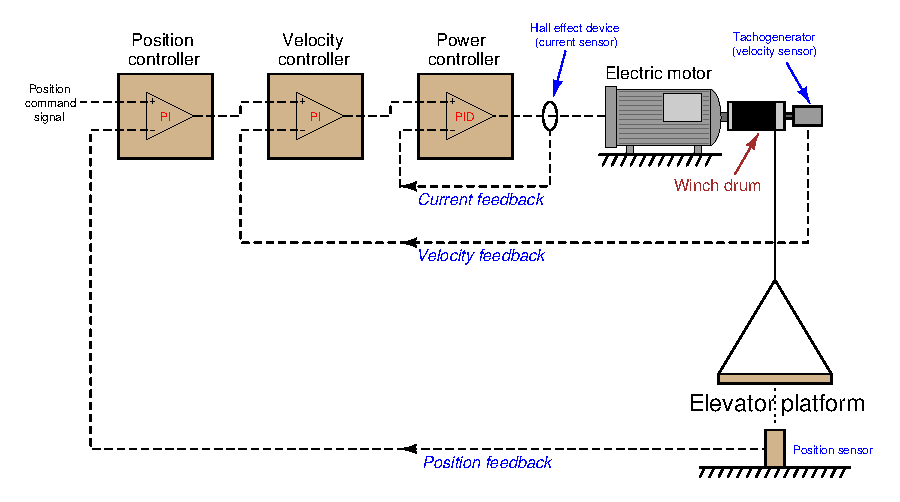
\includegraphics[height=7cm]{cont75.eps}$$
	\end{frame}

%
%Hypothetically, the position of the elevator could be controlled with a single PID controller sensing platform position and directly sending power to the motor.  However, much more precise control of the platform is achievable by sensing position, velocity, and motor current, and controlling each one of those variables with its own loop.  In motion control systems, each successive variable is the time-derivative of its precursor.  Velocity, for instance, is the time-derivative of position ($v = {dx \over dt}$).  Motor current, which is usually proportional to motor torque, which in turn is proportional to the angular acceleration ($\alpha$) of the winch and consequently the linear acceleration of the platform ($a$), is the time-derivative of velocity ($a = {dv \over dt}$).  If it were not for cascading, a single PID controller would have to control position by manipulating the \textit{acceleration} of the platform (i.e. motor current).  This would make the process characteristic ``runaway'' in nature, as any fixed amount of current will cause the platform to accelerate\footnote{At one specific current level, the motor will develop just enough torque to hold the platform's weight, at which point the acceleration will be zero.  Any amount of current above this value will cause an upward acceleration, while any amount of current below this value will cause a downward acceleration.}.
%
%Here with servomechanisms we see how cascading not only has the effect of ``shielding'' certain load variables from the master controller's view, but it also simplifies the dynamic characteristics of the process from that same point of view.  Instead of the position controller having to regulate an inherently ``runaway'' process, it now sees the process as having an ``integrating'' characteristic, since any constant output signal from the position controller results in the platform holding to a constant velocity (i.e. platform position will change at a constant rate over time, rather than at an accelerating rate).
%
%\vskip 10pt
%
%A necessary step in implementing cascade control is to ensure the secondary (``slave'') controller is well-tuned \textit{before} any attempt is made to tune the primary (``master'') controller.  Just a moment's thought is all that is needed to understand why this precedence in tuning must be: it is a simple matter of dependence.  The slave controller does not depend on good tuning in the master controller in order to control the slave loop.  If the master controller were placed in manual (effectively turning off its automatic response), the slave controller would simply control to a constant setpoint.  However, the master controller most definitely depends on the slave controller being well-tuned in order to fulfill the master's ``expectations.''  If the slave controller were placed in manual mode, the master controller would not be able to exert any control over its process variable whatsoever.  Clearly then, the slave controller's response is essential to the master controller being able to control its process variable, therefore the slave controller should be tuned first when initially commissioning or optimizing a cascade control system.
%
%\vskip 10pt
	\begin{frame}
		\frametitle{Modus for en kaskaderegulator}

		\begin{itemize}
			\item \textbf{Manuell modus} Regulatoren gjør ingenting automatisk, utgangen bestemmes av operatøren
			\item \textbf{Automatisk modus} Regulatoren prøver å holde PV=SP, SP settes manuelt av operatøren
			\item \textbf{Kaskade modus} Regulatoren prøver å holde PV=SP, SP settes av primær regulatoren og kalles ofte RSP. 
		\end{itemize}

		
	\end{frame}
	%
%Just like supervisory control systems where a process controller receives a ``remote'' setpoint signal from some other system, the secondary (``slave'') controller in a cascade system typically has three different operating modes:
%
%\begin{itemize}
%\item \textbf{Manual mode:} Controller takes no automatic action.  Output value set by human operator.
%\item \textbf{Automatic mode:} Controller automatically adjusts its output to try to keep PV = SP.  Setpoint value set ``locally'' by human operator.
%\item \textbf{Cascade mode:} Controller automatically adjusts its output to try to keep PV = SP.  Setpoint value set ``remotely'' by primary (master) controller.
%\end{itemize}
%
%This means it is possible to defeat a cascade control system by placing the secondary controller in the wrong mode (automatic) just as it is possible to defeat any control system by placing the controller in manual mode.  If a controller is ``slaved'' to another controller, it must be left in \textit{cascade} mode in order for the control strategy to function as designed.
%
%% ADD: discuss how cascaded flow systems may result in shifting the characteristics of a process from self-regulating (with lag) to purely integrating.
%
%
%
%
%
%
%
%
%
%
%
%\filbreak
%\section{Ratio control}
%
%Most people reading this book have likely had the experience of adjusting water temperature using two hand valves as they took a shower: one valve controlling the flow of hot water and the other valve controlling the flow of cold water.  In order to adjust water temperature, the \textit{proportion} of one valve opening to the other must be changed.  Increasing or decreasing total water flow rate without upsetting the outlet temperature is a matter of adjusting both valves in the same direction, maintaining that same proportion of hot to cold water flow.
%
%Although you may not have given it much thought while taking your shower, you were engaged in a control strategy known as \textit{ratio control}, where the ratio of one flow rate to another is controlled for some desired outcome.  Many industrial processes also require the precise mixing of two or more ingredients to produce a desired product.  Not only do these ingredients need to be mixed in proper proportion, but it is usually desirable to have precise control over the total flow rate as well.  \index{Ratio control strategy}
%
%A simple example of ratio control is in the production of paint, where a base liquid must be mixed with one or more pigments to achieve a desired consistency and color.  A manually controlled paint mixing process, similar to the hot and cold water valve ``process'' in some home showers, is shown here.  Two flowmeters, a ratio calculating relay, and a display provide the human operator with a live measurement of pigment-to-base ratio:
%
%$$\includegraphics{cont22.eps}$$
	\begin{frame}
		\frametitle{Forholdsregulering}

		$$\includegraphics[height=7cm]{cont22.eps}$$
	\end{frame}

	\begin{frame}
		\frametitle{Forholdsregulering}

		$$\includegraphics[height=7cm]{cont23.eps}$$
	\end{frame}
%
%\filbreak
%
%One alteration we could make to this mixing system is to link the two manual control valve handles together in such a way that the ratio of base to pigment was \textit{mechanically} established.  All the human operator needs to do now is move the one link to increase or decrease mixed paint production:
%
%$$\includegraphics{cont23.eps}$$
%
%Adjusting the pigment-to-base ratio is now a matter of adjusting the linkage ratio, a task most likely performed by a mechanic or someone else skilled in the alignment of mechanical linkages.  The convenience of total flow adjustment gained by the link comes at the price of inconvenient ratio adjustment.
%
%\filbreak
%
%Mechanical link ratio-control systems are commonly used to manage simple burners, proportioning the flow rates of fuel and air for clean, efficient combustion.  A photograph of such a system appears here, showing how the fuel gas valve and air damper motions are coordinated by a single rotary actuator:
%
%$$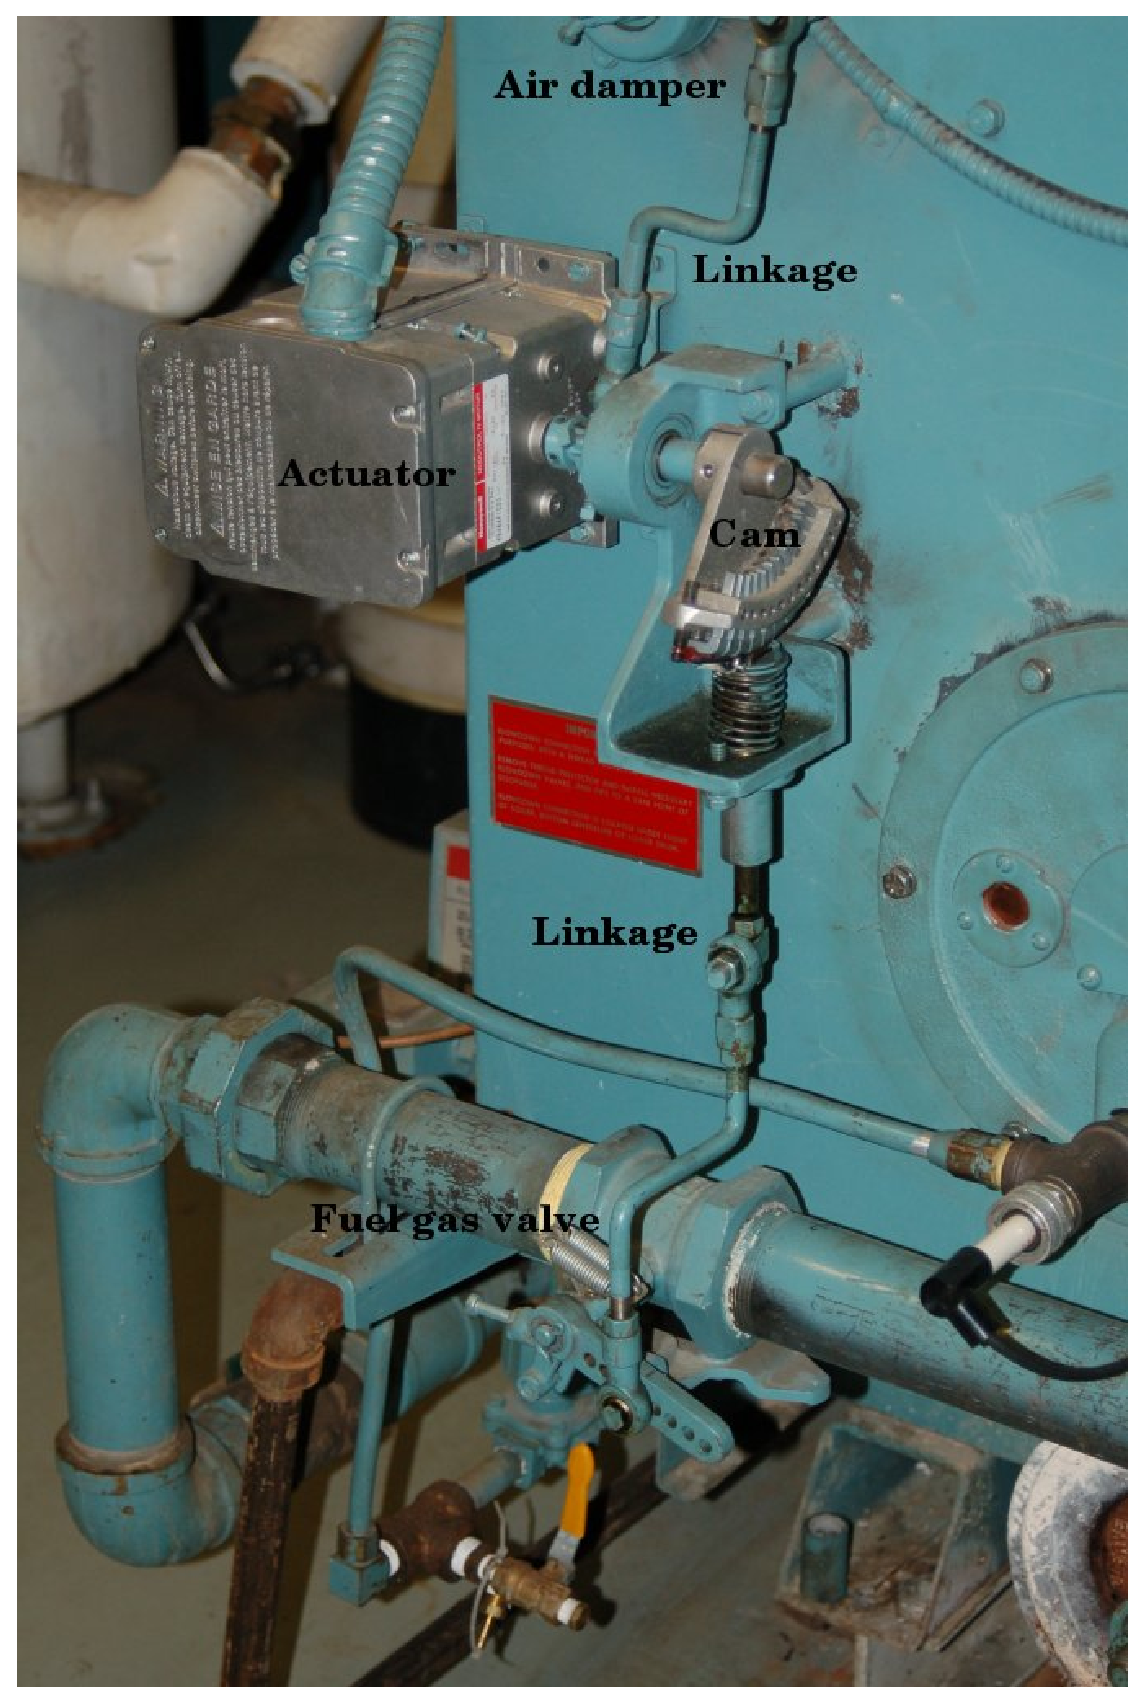
\includegraphics[width=4in]{cont67.eps}$$
	\begin{frame}
		\frametitle{Forholdsregulering}

		$$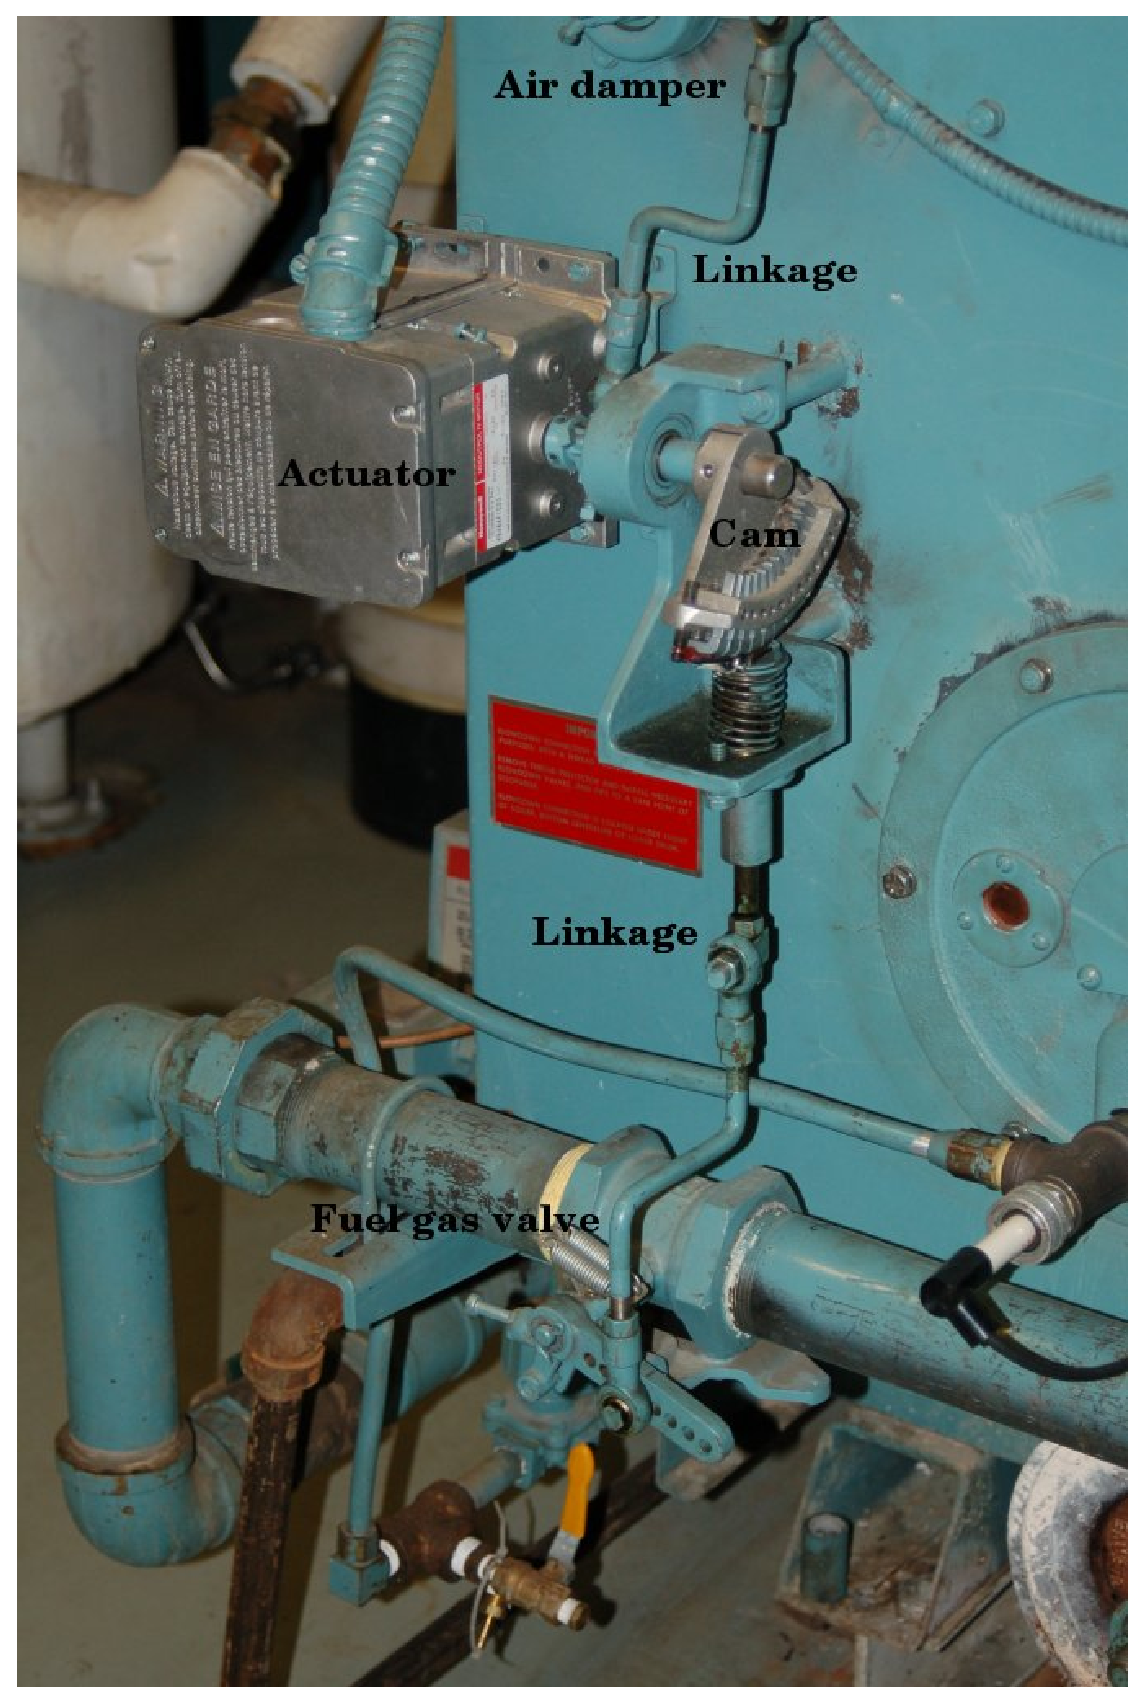
\includegraphics[height=7cm]{cont67.eps}$$
	\end{frame}
%
%As you can see in this photo, the fuel gas valve is actuated by means of a cam, allowing precise ``tuning'' of the valve characteristics for consistent fuel/air ratio across a wide range of firing rates.  Making ratio adjustments in such a linkage system is obviously a task for a skilled mechanic or technician.
%
%\filbreak
%
%A more automated approach to the general problem of ratio control involves the installation of a flow control loop on one of the lines and a flow-sensing transmitter on the other line.  The signal coming from the uncontrolled flow transmitter becomes the setpoint for the flow control loop:
%
%$$\includegraphics{cont24.eps}$$
	\begin{frame}
		\frametitle{Forholdsregulering}

		$$\includegraphics[height=7cm]{cont24.eps}$$
	\end{frame}
%
%Here, the flow transmitter on the uncontrolled line measures the flow rate of base, sending a flow rate signal to the pigment flow controller which acts to match flow rates.  If the calibrations of each flow transmitter are precisely equal to one another, the ratio of pigment to base will be 1:1 (equal).  The flow of base liquid into the mixing system is called a \textit{wild flow} or \textit{wild variable}, since this flow rate is not controlled by the ratio control system.  The only purpose served by the ratio control system is to match the pigment flow rate to the wild (base) flow rate, so the same ratio of pigment to base will always be maintained regardless of total flow rate.  Thus, the flow rate of pigment will be held \textit{captive} to match the ``wild'' base flow rate, which is why the controlled variable in a ratio system is sometimes called the \textit{captive variable} (in this case, a captive \textit{flow}).  \index{Wild variable}  \index{Wild flow}  \index{Captive variable}  \index{Captive flow}
%
%As with the mechanically-linked manual ratio mixing system, this ratio control system provides convenient total flow control at the expense of convenient ratio adjustment.  In order to alter the ratio of pigment to base, someone must re-range one or more flow transmitters.  To achieve a 2:1 ratio of base to pigment, for example, the base flow transmitter's range would have to be double that of the pigment flow transmitter.  This way, an equal percentage of flow registered by both flow transmitters (as the ratio controller strives to maintain equal percentage values of flow between pigment and base) would actually result in twice the amount of base flow than pigment flow.
%
%\filbreak
%
%We may incorporate convenient ratio adjustment into this system by adding another component (or function block) to the control scheme: a device called a \textit{signal multiplying relay} (or alternatively, a \textit{ratio station}).  This device (or computer function) takes the flow signal from the base (wild) flow transmitter and multiplies it by some constant value ($k$) before sending the signal to the pigment (captive) flow controller as a setpoint:  \index{Multiplying relay}  \index{Ratio station}
%
%$$\includegraphics{cont25.eps}$$
	\begin{frame}
		\frametitle{Forholdsregulering}

		$$\includegraphics[height=7cm]{cont25.eps}$$
	\end{frame}
%
%With identical flow range calibrations in both flow transmitters, this multiplying constant $k$ directly determines the pigment-to-base ratio (i.e. the ratio will be 1:1 when $k=1$; the ratio will be 2:1 when $k=2$, etc.).  If the $k$ value is easily adjusted by a human operator, mixing ratio becomes a very simple parameter to change at will, just as the total production rate is easy to adjust by moving the base flow control valve.
%
%\vskip 10pt
%
%Another example of ratio control at work is in a process whereby hydrocarbon gases (usually methane) are converted into hydrogen gas and carbon dioxide gas.  This is known as the \textit{steam-hydrocarbon reforming process}, and it is one of the more popular ways of generating hydrogen gas for industrial use.  The overall reaction for this process with methane gas (CH$_{4}$) and steam (H$_{2}$O) as the reactants is as follows\footnote{The conversion from hydrocarbon and steam to hydrogen and carbon dioxide is typically a two-stage process: the first (\textit{reforming}) stage produces hydrogen gas and carbon monoxide, while a second (\textit{water-gas-shift}) stage adds more steam to convert the carbon monoxide into carbon dioxide with more hydrogen liberated.  Both reactions are endothermic, with the reforming reaction being more endothermic than the water-gas-shift reaction.}:  \index{Steam-hydrocarbon reforming process}
%
%$$\hbox{CH}_4 + 2\hbox{H}_2\hbox{O} \to 4\hbox{H}_2 + \hbox{CO}_2$$
%
%This is an \textit{endothermic chemical reaction}, which means a net input of energy is required to make it happen.  Typically, the hydrocarbon gas and steam are mixed together in a heated environment in the presence of a catalyst (to reduce the activation energy requirements of the reaction).  This usually takes the form of catalyst-packed metal tubes inside a gas-fired furnace.  It is important to control the proportion of gas to steam flow into this process.  Too much hydrocarbon gas, and the result will be ``coking'' (solid hydrocarbon deposits) inside the heated tubes and on the surface of the catalyst beads, decreasing the efficiency of the process over time.  Too much steam and the result is wasted energy as unreacted steam simply passes through the heater tubes, absorbing heat and carrying it away from the catalyst where it would otherwise do useful work.
%
%One way to achieve the proper ratio of hydrocarbon gas to steam flow is to install a normal flow control loop on one of these two reactant feed lines, then use that process variable (flow) signal as a setpoint to a flow controller installed on the other reactant feed line.  This way, the second controller will maintain a proper balance of flow to proportionately match the flow rate of the other reactant.  An example P\&ID is shown here, where the methane gas flow rate establishes the setpoint for steam flow control:
%
%$$\includegraphics{cont20.eps}$$
	\begin{frame}
		\frametitle{Forholdsregulering}

$$\hbox{CH}_4 + 2\hbox{H}_2\hbox{O} \to 4\hbox{H}_2 + \hbox{CO}_2$$
		$$\includegraphics[height=7cm]{cont20.eps}$$
	\end{frame}
%
%Note how the methane gas flow transmitter signal goes both to the methane flow controller and to a \textit{multiplying relay} that multiplies this signal by a constant value ($k$) before passing it on to the steam flow controller as a setpoint.  This $k$ value sets the \textit{ratio} of steam flow to methane flow.  Although this might appear to be a cascade control system at first glance, it is actually quite different.  In a cascade system, the \textit{output} of one controller becomes the setpoint for another.  Here in a ratio control system, the \textit{process variable} of one controller becomes the setpoint for another, such that two process variables remain in constant proportion (ratio) to one another.
%
%If the two flow transmitters are compensated to measure mass flow, the ideal value of $k$ should be set such that two molecules of steam vapor (H$_{2}$O) enter the reforming furnace for every one molecule of methane (CH$_{4}$).  With a 2-to-1 molecular ratio of steam to methane (2 moles of steam per one mole of methane), this equates to a 9-to-4 mass flow ratio once the formula weights of steam and methane are calculated\footnote{Steam has a formula weight of 18 amu per molecule, with two hydrogen atoms (1 amu each) and one oxygen atom (16 amu).  Methane has a formula weight of 16 amu per molecule, with one carbon atom (12 amu) and four hydrogen atoms (1 amu each).  If we wish to have a molecular ratio of 2:1, steam-to-methane, this makes a formula weight ratio of 36:16, or 9:4.}.  Thus, if the methane and gas flowmeters are calibrated for equal mass flow ranges, the ideal value for $k$ should be ${9 \over 4}$, or 2.25.  Alternatively, the flow transmitter calibrations could be set in such a way that the ideal ratio is intrinsic to those transmitters' ranges (i.e. the methane flow transmitter has 2.25 times the mass flow range of the steam flow transmitter), with $k$ set to an ideal value of 1.  This way a 9:4 ratio of methane mass flow to steam mass flow will result in equal percentage output values from both flow transmitters.  In practice, the value for $k$ is set a bit higher than ideal, in order to ensure just a little excess steam to guard against coking inside the reaction heater tubes\footnote{It is quite common for industrial control systems to operate at ratios a little bit ``skewed'' from what is stoichiometrically ideal due to imperfect reaction efficiencies.  Given the fact that no chemical reaction ever goes to 100\% completion, a decision must be made as to which form of incompleteness is worse.  In a steam-hydrocarbon reforming system, we must ask ourselves which is worse: excess (unreacted) steam at the outlet, or excess (unreacted) hydrocarbon at the outlet.  Excess hydrocarbon content will ``coke'' the catalyst and heater tubes, which is very bad for the process over time.  Excess steam merely results in a bit more operating energy loss, with no degradation to equipment life.  The choice, then, is clear: it is better to operate this process ``hydrocarbon-lean'' (more steam than ideal) than ``hydrocarbon-rich'' (less steam than ideal).}.  \index{Formula weight}
%
%\filbreak
%
%We could add another layer of sophistication to this ratio control system by installing a gas analyzer at the outlet of the reaction furnace designed to measure the composition of the product stream.  This analyzer's signal could be used to adjust the value of $k$ so the ratio of steam to methane would automatically vary to ensure optimum production quality even if the feedstock composition (i.e. percentage concentration of methane in the hydrocarbon gas input) changes:
%
%$$\includegraphics{cont21.eps}$$
	\begin{frame}
		\frametitle{Forholdsregulering}

$$\hbox{CH}_4 + 2\hbox{H}_2\hbox{O} \to 4\hbox{H}_2 + \hbox{CO}_2$$
		$$\includegraphics[height=7cm]{cont21.eps}$$
	\end{frame}
%
%As we saw before, pure methane feed requires a 9-to-4 steam-to-methane mass flow ratio for the desired reaction to be stoichiometrically balanced.  This mass ratio, however, is not balanced for hydrocarbons other than methane.  Ethane (C$_{2}$H$_{6}$) processed in the same way requires a 12-to-5 steam-to-ethane mass flow ratio.  Propane (C$_{3}$H$_{8}$) requires a 26-to-11 steam-to-propane mass flow ratio.  If the hydrocarbon feed to the reforming furnace varies in composition, the steam flow ratio ($k$) must change accordingly for efficient reaction.
%
%
%
%
%
%
%
%
%\filbreak
%\section{Relation control}
%
%A control strategy similar to ratio control is \textit{relation} control.  This is similar to ratio control in that a ``wild'' variable determines the setpoint for a captive variable, but with relation control the mathematical relationship between the wild and captive variables is one of addition (or subtraction) rather than multiplication (or division).  In other words, a relation control system works to maintain a specific \textit{difference} between wild and captive flow values, whereas a ratio control system works to maintain a specific \textit{ratio} between wild and captive flow values.  \index{Relation control strategy}
%
%An example of relation control appears here, where a temperature controller for a steam superheater on a boiler receives its setpoint from the biased output of a temperature transmitter sensing the temperature of saturated steam (that is, steam exactly at the boiling point of water) in the steam drum:
%
%$$\includegraphics{cont70.eps}$$
	\begin{frame}
		\frametitle{Regulering av sammenheng i dampkjele}

		$$\includegraphics[height=7cm]{cont70.eps}$$
	\end{frame}

%
%It is a basic principle of thermodynamics that the vapor emitted at the surface of a boiling liquid will be at the same temperature as that liquid.  Furthermore, any heat lost from that vapor will cause at least some of that vapor to condense back into liquid.  In order to ensure the vapor is ``dry'' (i.e. it may lose substantial heat energy without condensing), the vapor must be heated beyond the liquid's boiling point at some later stage in the process.
%
%Steam within the steam drum of a boiler is \textit{saturated} steam: at the same temperature as the boiling water.  Any heat lost from saturated steam causes at least some of it to immediately condense back into water.  In order to ensure ``dry'' steam output from the boiler, the saturated steam taken from the steam drum must be further heated through a set of tubes called a \textit{superheater}.  The resulting ``dry'' steam is said to be \textit{superheated}, and the difference between its temperature and the temperature of the boiling water (saturated steam) is called \textit{superheat}.  \index{Superheater}  \index{Superheat}  \index{Superheated steam}
%
%This control system maintains a set amount of superheat by measuring the saturated steam's temperature (within the steam drum), adding a ``superheat setpoint'' bias value to that signal, then passing the biased signal to the temperature indicating controller (TIC) where the superheated steam temperature is regulated by adding water\footnote{This mixing of superheated steam and cold water happens in a specially-designed device called a \textit{desuperheater}.  The basic concept is that the water will absorb heat from the superheated steam, turning that injected water completely into steam and also reducing the temperature of the superheated steam.  The result is a greater volume of steam than before, at a reduced temperature.  So long as some amount of superheat remains, the de-superheated steam will still be ``dry'' (above its condensing temperature).  The desuperheater control merely adds the appropriate amount of water until it achieves the desired superheat value.} to the superheated steam.  With this system in place, the boiler operator may freely define how much superheat is desired, and the controller attempts to maintain the superheated steam at that much higher temperature than the saturated steam in the drum, over a wide range of saturated steam temperatures.  \index{Desuperheater}
%
%A ratio control system would not be appropriate here, since what we desire in this process is a controlled \textit{offset} (rather than a controlled \textit{ratio}) between two steam temperatures.  The control strategy looks very much like a ratio control, except for the substitution of a summing function instead of a multiplying function.
%
%
%
%
%
%
%
%
%\filbreak
%\section{Feedforward control}
%
%``Feedforward'' is a rather under-used control strategy capable of managing a great many types of process problems.  It is based on the principle of \textit{preemptive load counter-action:} that if all significant loads on a process variable are monitored, and their effects on that process variable are well-understood, a control system programmed to take appropriate action based on load changes will shield the process variable from any ill effect.  That is to say, the feedforward control system uses data from load sensors to predict when an upset is about to occur, then \textit{feeds that information forward to the final control element} to counteract the load change before it has an opportunity to affect the process variable.  Feedback control systems are \textit{reactive}, taking action after to changes in the process variable occur.  Feedforward control systems are \textit{proactive}, taking action before changes to the process variable can occur.
%
%This photograph shows a kind of feedforward strategy employed by human operators running a \textit{retort}: a steam-powered machine used to pressure-treat wooden beams at a milled lumber operation.  The sign taped to this control panel reminds the operator to warn the maintenance department of an impending steam usage:
%
%$$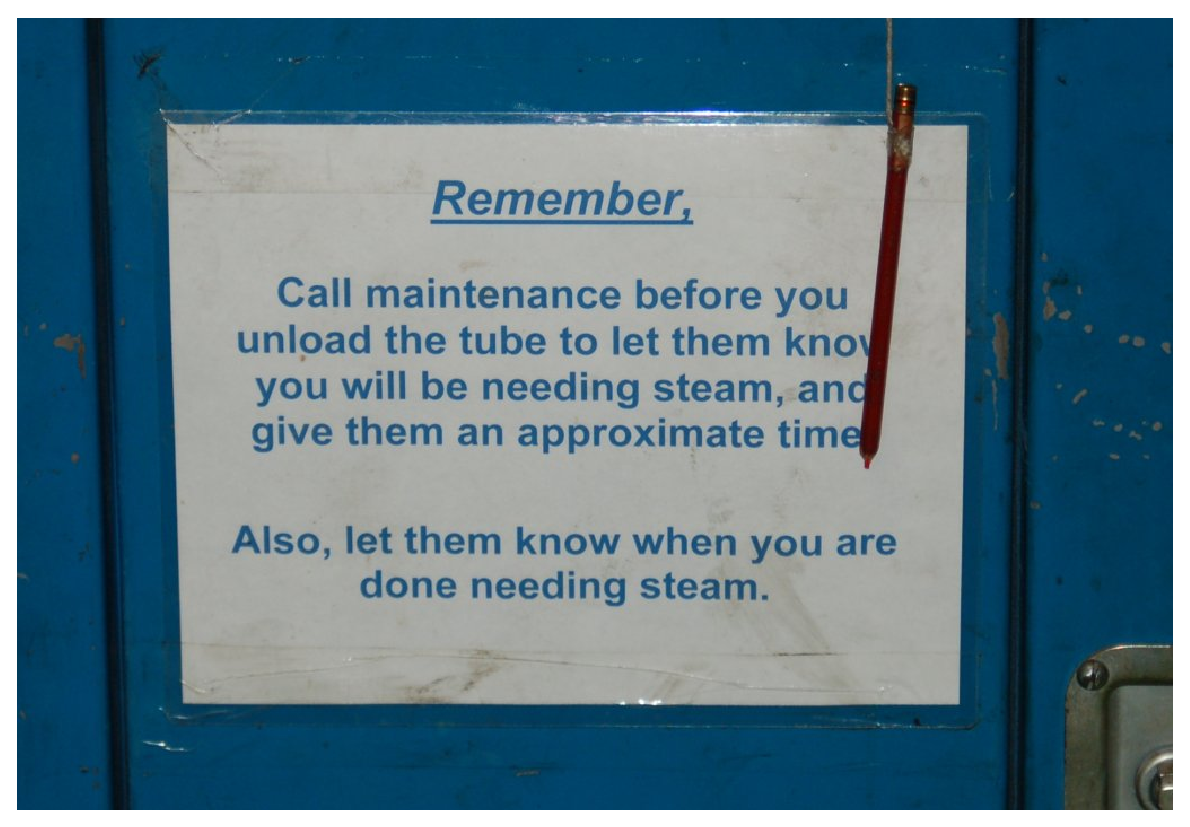
\includegraphics[width=5in]{cont86.eps}$$
	\begin{frame}
		\frametitle{Foroverkoblet regulering}

		$$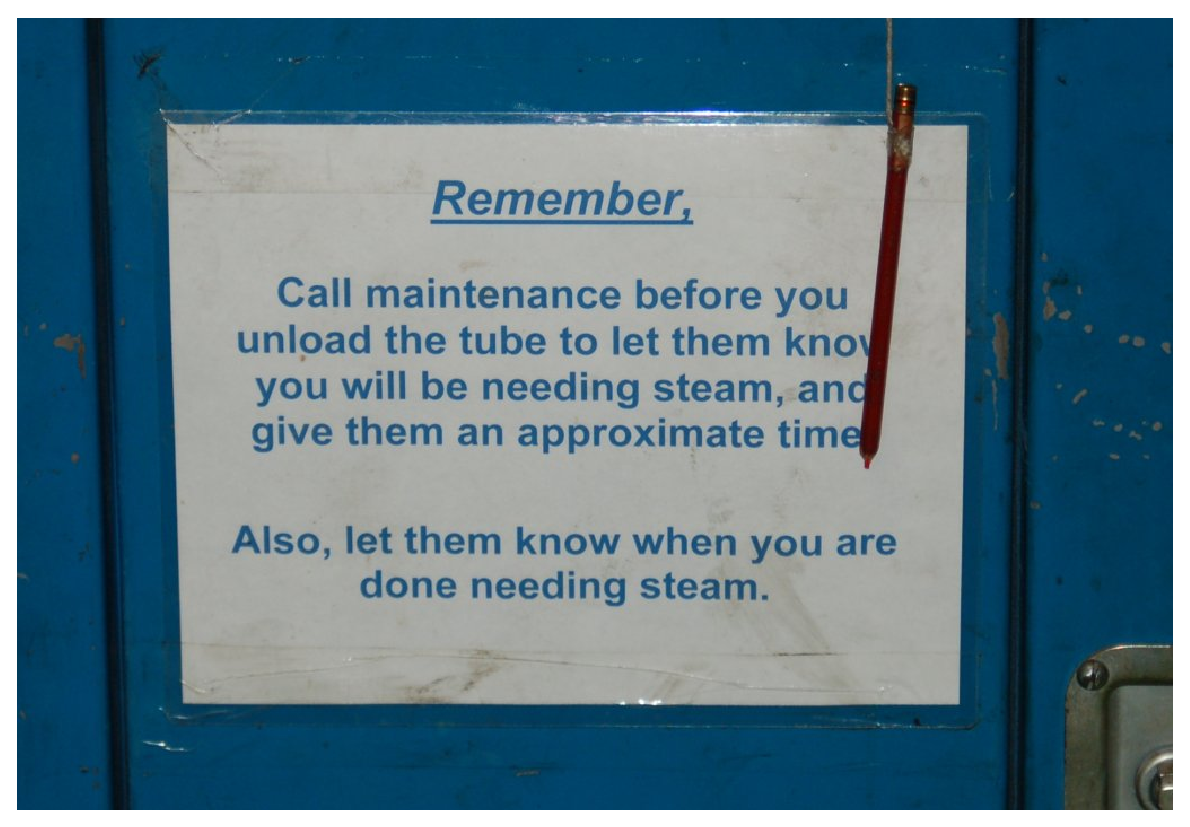
\includegraphics[height=7cm]{cont86.eps}$$
	\end{frame}

%
%The story behind this sign is that a sudden demand in retort steam causes the entire facility's steam supply pressure to sag if it happens at a time when the boiler is idling.  Since the boiler's pressure control system can only react to deviations in steam pressure from setpoint, the boiler pressure controller will not take any action to compensate for sudden demand until \textit{after} it sees the steam pressure fall, at which point it may be too late to fully recover.  If operators give the maintenance personnel advance notice of the steam demand, though, the boiler may be fired up for extra steam capacity and thus will be prepared for the extra demand when it comes.  The upset avoided here is abnormally low steam header pressure, with the predictive load being the retort operator's planned usage of steam.  Crude as this solution might be, it illustrates the fundamental concept of feedforward control: information about a load change is ``fed forward'' to the final control element to preemptively stabilize the process variable.
%
%\vskip 10pt
%
%As the following section explains, perfect feedforward control action is nearly impossible to achieve.  However, even imperfect feedforward action is often far better than none at all, and so this control strategy is quite valuable in process control applications challenged by frequent and/or large variations in load.
%
%
%
%
%
%\filbreak
%\subsection{Load Compensation}
%
%\textit{Feedback} control works on the principle of information from the outlet of a process being ``fed back'' to the input of that process for corrective action.  A block diagram of feedback control looks like a loop:  \index{Feedback control system}
%
%$$\includegraphics{cont05.eps}$$
	\begin{frame}
		\frametitle{Belastningskompensering}

		$$\includegraphics[height=7cm]{cont05.eps}$$
	\end{frame}

%
%\filbreak
%
%The reason any control system is necessary at all\footnote{This statement is true only for self-regulating processes.  Integrating and ``runaway'' processes require control systems to achieve stability even in the complete absence of any loads.  However, since self-regulation typifies the vast majority of industrial processes, we may conclude that the fundamental purpose of most control systems is to counteract the effects of loads.} to maintain a process variable at some stable value is the existence of something called a \textit{load}.  A ``load'' is a variable influencing a process that is not itself under direct control, and may be represented in the block diagram as an arrow entering the process, but not within the control loop:  \index{Load, process}  \index{Process load}
%
%$$\includegraphics{cont26.eps}$$
	\begin{frame}
		\frametitle{Belastningskompensering}

		$$\includegraphics[height=7cm]{cont26.eps}$$
	\end{frame}
%
%For example, consider the problem of controlling the speed of an automobile.  In this scenario, vehicle speed is the process variable being measured and controlled, while the final control device is the accelerator pedal controlling engine power output.  If it were not for the existence of hills and valleys, head-winds and tail-winds, air temperature changes, road surface variations, and a host of other ``load'' variables affecting car speed, maintaining a constant speed would be as simple as holding the accelerator pedal at a constant position.
%
%However, the presence of these ``load'' variables makes necessitates a human driver (or a \textit{cruise control} system) continually adjusting engine power to maintain constant speed.  Using the car's measured speed as feedback, the driver (or cruise control) adjusts the accelerator pedal position as necessary based on whether or not the car's speed matches the desired ``setpoint'' value.
%
%An inherent weakness of any feedback control system is that it can never be \textit{proactive}.  The best any feedback control system can ever do is \textit{react} to detected disturbances in the process variable.  This makes deviations from setpoint inevitable, even if only for short periods of time.  In the context of our automobile cruise control system, this means the car can never maintain a \textit{perfectly} constant speed in the face of loads because the control system does not have the ability to anticipate loads (e.g. hills, wind gusts, changes in air temperature, changes in road surface, etc.).  At best, all the feedback cruise control system can do is react to changes in speed it senses \textit{after} some load has disturbed it.
%
%\vskip 10pt
%
%\textit{Feedforward} control addresses this weakness by taking a fundamentally different approach, basing final control decisions on the states of load variables rather than the process variable.  In other words, a feedforward control system monitors the factor(s) influencing a process and decides how to compensate \textit{ahead of time} before the process variable deviates from setpoint.  If all loads are accurately measured, and the control algorithm realistic enough to predict process response for these known load values, the process variable (ideally) need not be measured at all:  \index{Feedforward control strategy}
%
%$$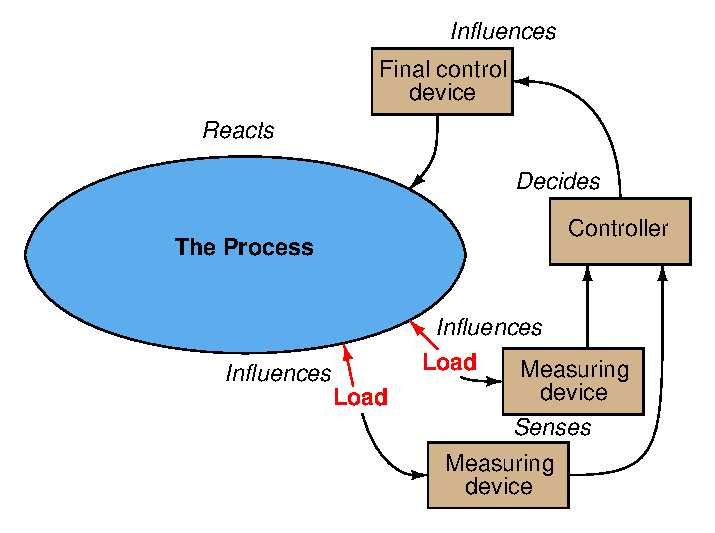
\includegraphics{cont27.eps}$$
	\begin{frame}
		\frametitle{Belastningskompensering}

		$$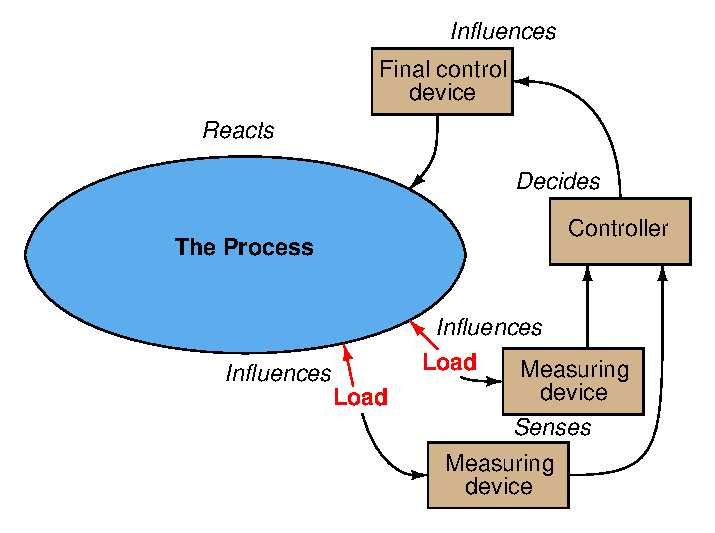
\includegraphics[height=7cm]{cont27.eps}$$
	\end{frame}
%
%As was the case with cascade control, feedforward control also has an analogue in workplace management.  If you consider a supervisor to be the ``controller'' of a work group (issuing orders to his or her subordinates to accomplish important tasks), a feedforward system would be when someone informs the supervisor of an important change that will soon impact the work group.  By having this information ``fed forward'' to the supervisor, the supervisor may then take \textit{preemptive} measures to better manage this change before its effects are fully felt.  If this predictive information is accurate, and the supervisor's response appropriate, any negative impacts of the change will be minimized to the point where no reactive steps will be needed.  Stated differently, good feedforward control action translates what would otherwise be a crisis into an insignificant event.
%
%Returning to the cruise control application, a purely feedforward automobile cruise control system would be interfaced with topographical maps, real-time weather monitors, and road surface sensors to decide how much engine power was necessary at any given time to attain the desired speed\footnote{The load variables I keep mentioning that influence a car's speed constitute an incomplete list at best.  Many other variables come into play, such as fuel quality, engine tuning, and tire pressure, just to name a few.  In order for a purely feedforward (i.e. no feedback monitoring of the process variable) control system to work, \textit{every single load variable} must be accurately monitored and factored into the system's output signal.  This is impractical or impossible for a great many applications, which is why we usually find feedforward control used in conjunction with feedback control, rather than feedforward control used alone.}.  Assuming all relevant load variables are accounted for, the cruise control would be able to maintain constant speed regardless of conditions, and without the need to even monitor the car's speed.
%
%This is the promise of feedforward control: a method of controlling a process variable so perfect in its predictive power that it eliminates the need to even measure that process variable.  If you are skeptical of this feedforward principle and its ability to control a process variable without even measuring it, this is a good thing -- you are thinking critically!  In practice, it is nearly impossible to accurately account for \textit{all} loads influencing a process and to both anticipate and counter-act their combined effects, and so \textit{pure} feedforward control systems are rare\footnote{In fact, the only pure feedforward control strategies I have ever seen have been in cases where the process variable was nearly impossible to measure and could only be inferred from other variables.}.  Instead, the feedforward principle finds use as a supplement to normal feedback control.  To understand feedforward control better, however, we will consider its pure application before exploring how it may be combined with feedback control.
%
%\vskip 10pt
%
%\filbreak
%
%First, let us consider a liquid level control system on an open tank, where three different fluid ingredients (shown in the following P\&ID simply as A, B, and C) are mixed to produce a final product.  A level transmitter (LT) measures liquid level, while a level controller (LC) compares this level to a setpoint value, and outputs a signal calling for a certain amount of discharge flow.  A cascaded (slave) flow controller (FC) senses outgoing flow via a flow transmitter (FT) and works to maintain whatever rate of flow is ``asked'' for by the level controller:
%
%$$\includegraphics{cont28.eps}$$
	\begin{frame}
		\frametitle{Foroverkoblet regulering}

		$$\includegraphics[height=7cm]{cont28.eps}$$
	\end{frame}
%
%The level control system acts to keep liquid level constant in the vessel, ensuring adequate mixing of the three ingredients\footnote{If the liquid level drops too low, there will be insufficient \textit{retention time} in the vessel for the fluids to mix before they exit the product line at the bottom.}.  Being a feedback level control system, it adjusts the discharge flow rate in response to measured changes in liquid level.  Like all feedback control systems, this one is \textit{reactive} in nature: it can only take corrective action \textit{after} a deviation between process variable (level) and setpoint is detected.  As a result, temporary deviations from setpoint are guaranteed to occur with this control system every time the combined flow rate of the three ingredients increases or decreases.  \index{Retention time}
%
%Let us now change the control system strategy from feedback to feedforward.  It is clear what the loads are in this process: the three ingredient flows entering the vessel.  If we measure and sum these three flow rates\footnote{The device or computer function performing the summation is shown in the P\&ID as a bubble with ``FY'' as the label.  The letter ``F'' denotes \textit{Flow}, while the letter ``Y'' denotes a signal relay or transducer.}, then use the total incoming flow signal as a setpoint for the discharge flow controller, the outlet flow should (ideally) match the inlet flow, resulting in a constant liquid level.  Being a purely feedforward control system, there is no level transmitter (LT) any more, just flow transmitters measuring the three loads:
%
%$$\includegraphics{cont29.eps}$$
	\begin{frame}
		\frametitle{Foroverkoblet regulering}

		$$\includegraphics[height=7cm]{cont29.eps}$$
	\end{frame}
%
%If all flow transmitter calibrations are perfect, the summing of flow rates flawless, and the flow controller's tuning robust, this level control system should control liquid level in the vessel by proactive effort (``thinking ahead'') rather than reactive effort (``after the fact'').  Any change in the flow rate of ingredients A, B, and/or C is quickly matched by an equal adjustment to the discharge flow rate.  So long as total volumetric flow out of the vessel is held equal to total volumetric flow into the vessel, the liquid level inside the vessel \textit{cannot} change\footnote{Incidentally, this is a good example of an \textit{integrating} mass-balance process, where the rate of process variable change over time is proportional to the imbalance of flow rates in and out of the process.  Stated another way, total accumulated (or lost) mass in a mass-balance system such as this is the time-integral of the difference between incoming and outgoing mass flow rates: $\Delta m = \int_0^T (W_{in} - W_{out}) \> dt$.}.
%
%If this feedforward strategy reminds you of ratio control, you are thinking correctly: the ingredient flow sum signal is the \textit{wild variable}, and the discharge flow signal is the \textit{captive variable}.  The flow controller simply maintains the discharge flow rate at a 1:1 ratio with the (total) ingredient flow rate.  In fact, pure feedforward control is a variation of 1:1 ratio control, except that the real process variable (tank level) is neither the wild (total incoming flow) nor the captive variable (discharge flow) in the process.
%
%\vskip 10pt
%
%An interesting property of feedforward and ratio control systems alike is that they cannot generate oscillations as is the case with an over-tuned (excessive gain) feedback system.  Since a feedforward system does not monitor the effects of its actions, it cannot react to something it did to the process, which is the root cause of feedback oscillation.  While it is entirely possible for a feedforward control system to be configured with too much gain, the effect of this will be \textit{overcompensation} for a load change rather than oscillation.  In the case of the mixing tank feedforward level control process, improper instrument scaling and/or offsets will merely cause the discharge and inlet flows to mis-match, resulting in a liquid level that either continues to increase or decrease over time (``integrate'').  However, no amount of mis-adjustment can cause this feedforward system to produce \textit{oscillations} in the liquid level.
%
%In reality, this pure feedforward control system is impractical even if all instrument calibrations and control calculations are perfect.  There are still loads unaccounted for: evaporation of liquid from the vessel, for example, or the occasional pipe fitting leak.  Furthermore, since the control system has no ``knowledge'' of the actual liquid level, it cannot make adjustments to that level.  If an operator, for instance, desired to decrease the liquid level in order to reduce the residence time (also known as ``retention time'')\footnote{\textit{Residence time} or \textit{Retention time} is the average amount of time each liquid molecule spends inside the vessel.  It is an important variable in chemical reaction processes, where adequate time must be given to the reactant molecules in order to ensure a complete reaction.  It is also important for non-reactive mixing processes such as paint and food manufacturing, to ensure the ingredients are thoroughly mixed together and not stratified.  For any given flow rate through a vessel, the residence time is directly proportional to the volume of liquid contained in that vessel: double the captive volume, and you double the residence time.  For any given captive volume, the residence time is inversely proportional to the flow rate through the vessel: double the flow rate through the vessel, and you halve the residence time.  In some mixing systems where residence time is critical to the thorough mixing of liquids, vessel level control may be coupled to measured flow rate, such that an increase in flow rate results in an increased level setpoint, thus maintaining a constant residence time despite changes in production rate.}, he or she would have to manually drain liquid out of the vessel, or temporarily place the discharge flow controller in ``manual'' mode and increase the flow there (then place back into ``cascade'' mode where it follows the remote setpoint signal again).  The advantage of proactive control and minimum deviation from setpoint over time comes at a fairly high price of impracticality and inconvenience.  \index{Retention time}  \index{Residence time, see Retention time}
%
%\filbreak
%
%For these reasons, feedforward control is most often found in conjunction with feedback control.  To show how this would work in the liquid level control system, we will incorporate a level transmitter and level controller back into the system, the output of that level controller being summed with the feedforward flow signal (by the LY summing relay) before going to the cascaded setpoint input of the discharge flow controller:
%
%$$\includegraphics{cont30.eps}$$
	\begin{frame}
		\frametitle{Foroverkoblet regulering}

		$$\includegraphics[height=7cm]{cont30.eps}$$
	\end{frame}
%
%This hybrid control strategy is sometimes called \textit{feedforward with trim}.  In this context, ``trim'' refers to the level controller's (LC) output signal contributing to the discharge flow setpoint, helping to compensate for any unaccounted loads (evaporation, leaks) and provide for level setpoint changes.  This ``trim'' signal should do very little of the control work in this system, the bulk of the liquid level stability coming from the feedforward signals provided by the incoming flow transmitters.  \index{Feedforward with trim}  \index{Trim, in a feedforward control system}
%
%%\filbreak
%
%% ADD: elaborate on feedforward with trim versus ratio with trim.
%
%%Recall how pure feedforward control in its simplest form (having no feedback) was likened to a ratio control system with a fixed 1:1 ratio.  With the addition of feedback (trim) to feedforward, we see something that is truly different from what ratio control looked like with the addition of feedback.  In a ratio control system having feedback, the feedback altered the ratio between wild and captive variables.  In a feedforward control system, the feedback merely \textit{offsets} the wild and captive variables.  Using functional diagrams to illustrate:
%
%%$$\includegraphics{.eps}$$
%
%\filbreak
%
%A very similar control strategy commonly used on large steam boilers for the precise control of steam drum water level goes by the name of \textit{three-element feedwater control}.  The following illustration shows an example of this control strategy implemented with pneumatic (3-15 PSI signal) instruments:  \index{Three-element boiler feedwater control}  \index{3-element boiler feedwater control}  \index{Three-element boiler feedwater control}
%
%$$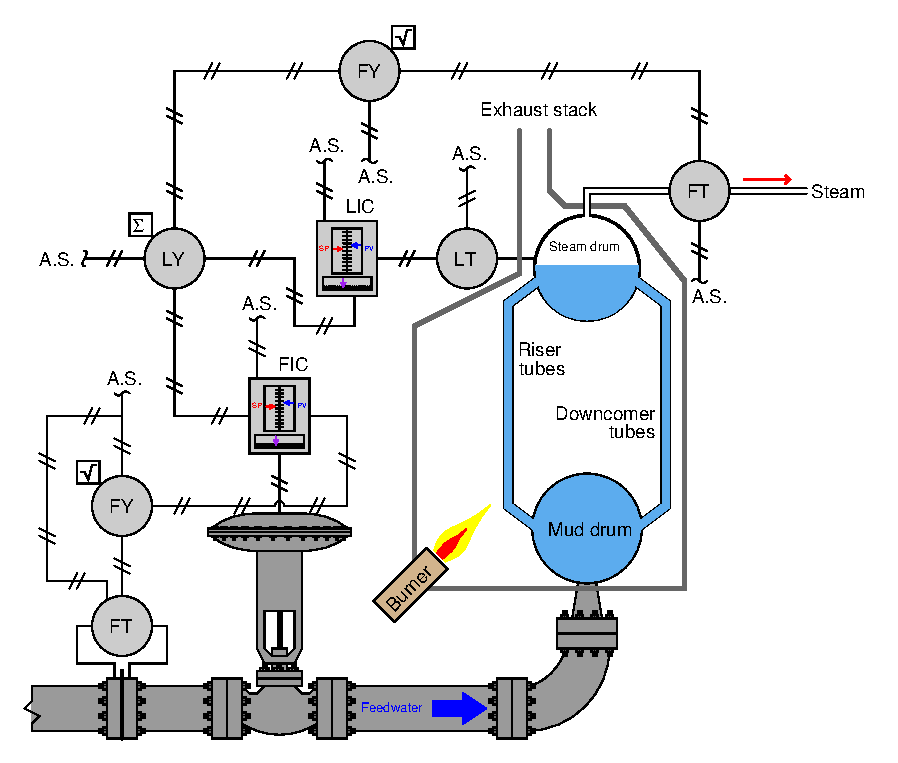
\includegraphics{cont31.eps}$$
	\begin{frame}
		\frametitle{Tre Elements regulering}

		$$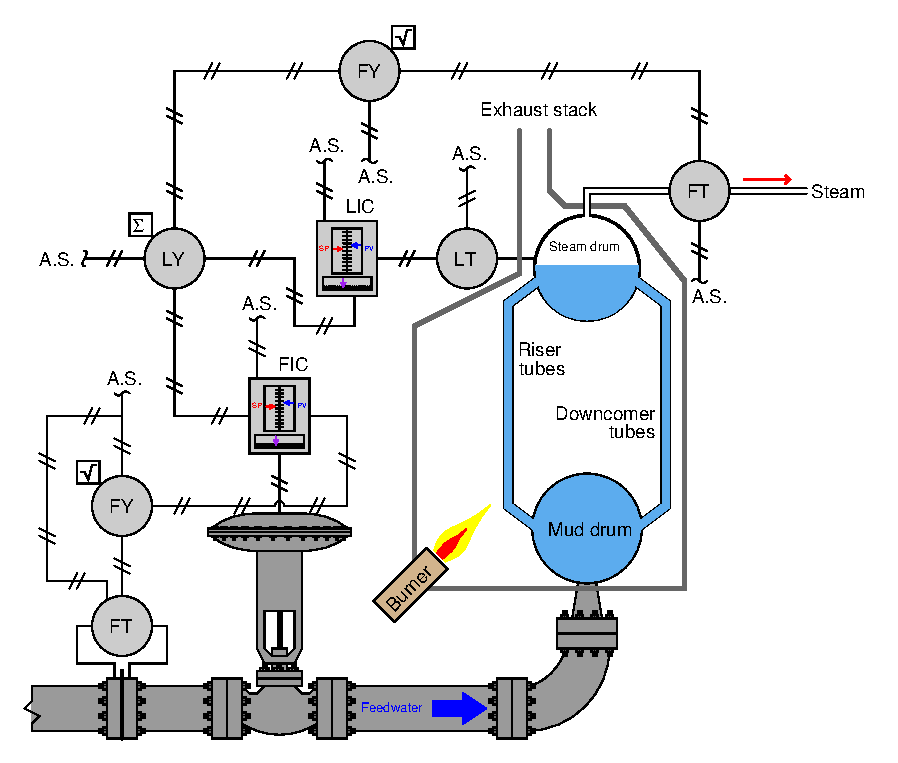
\includegraphics[height=7cm]{cont31.eps}$$
	\end{frame}
%
%Such a control system is called ``three-element'' because it makes use of three process measurements:
%
%\begin{itemize}
%\item Feedwater flow rate
%\item Steam drum water level
%\item Steam flow rate
%\end{itemize}
%
%Feedwater flow is controlled by a dedicated flow controller (FIC), receiving a remote setpoint signal from a summing relay (LY).  The summer receives two inputs: a steam flow signal and the output signal (trim) from the level controller (LIC).  The feedforward portion of this system (steam flow feeding forward to water flow) is intended to match the mass flow rates of water into the boiler with steam flow out of the boiler.  If steam demand suddenly increases, this feedforward portion of the system immediately calls for a matching increase in water flow into the boiler, since every molecule of steam exiting the boiler must come from one molecule of water entering the boiler.  The level controller and transmitter act as a feedback control loop, supplementing the feedforward signal to the cascaded water flow controller to make up for (``trim'') any shortcomings of the feedforward loop.
%
%\vskip 10pt
%
%A three-element boiler feedwater control system is a good example of a feedforward strategy designed to ensure \textit{mass balance}, defined as a state of equality between all incoming mass flow rates and all outgoing mass flow rates.  The steam flow transmitter measures outgoing mass flow, its signal being used to adjust incoming water mass rate.  Since mass cannot be created or destroyed (the Law of Mass Conservation), every unit of steam mass leaving the boiler must be accounted for as an equivalent unit of water mass entering the boiler.  If the control system perfectly balances these mass flow rates, water level inside the boiler \textit{cannot} change.  \index{Mass balance}  \index{Conservation of Mass} 
%
%In processes where the process variable is affected by energy flow rates rather than mass, the balance maintained by a feedforward control system will be \textit{energy balance} rather than mass balance.  Like mass, energy cannot be created or destroyed (the Law of Energy Conservation), but must be accounted for.  A feedforward control system monitoring all incoming energy flows into a process and adjusting the outgoing energy flow rate (or vice-versa) will ensure no energy is depleted from or accumulated within the process, thus ensuring the stability of the processes' internal energy state.   \index{Energy balance}  \index{Conservation of Energy}
%
%\filbreak
%
%An example of energy-balance feedforward control appears in this heat exchanger temperature control system:
%
%$$\includegraphics{cont69.eps}$$
	\begin{frame}
		\frametitle{Foroverkoblet reguleringssystem basert på energibalanse}

		$$\includegraphics[height=7cm]{cont69.eps}$$
	\end{frame}

%
%The two transmitters on the incoming (cold oil) line measure oil temperature and oil flow rate, respectively.  The first ``summing'' function subtracts the incoming oil temperature from the setpoint (desired) temperature, and then the difference of these two temperatures is then multiplied by the flow rate signal to produce a signal representing the \textit{energy demand}\footnote{Energy demand is an example of what is called an \textit{inferred variable}: a physical quantity that we cannot measure directly but instead calculate from measurements made of other variables.} of the incoming oil (i.e. how much energy will be required to elevate the oil flow's temperature to setpoint).  The ``energy demand'' signal is summed with the temperature controller's output signal to set the steam valve position (adding energy to the process).  \index{Inferred variable}
%
%There do exist other loads in this process, such as ambient air temperature and chemical composition of the oil, but these variables are generally less influential on discharge temperature than feed temperature and flow rate.  This illustrates a practical facet of feedforward control: although there may be a great many loads affecting our process variable, we must generally limit our application of feedforward to only the most dominant loads in order to limit control system cost.  Simply put, we usually cannot justify the expense and complexity of a feedforward control system compensating for \textit{every single load} in a system.
%
%
%
%
%\filbreak
%\subsection{Proportioning feedforward action}
%
%Feedforward control works by directly modulating the manipulated variable in a control system according to changes sensed in the load(s).  In order for feedforward to function optimally, it must adjust the manipulated variable in a manner that is proportionate to the need: no more, and no less.  At this juncture it is appropriate to ask the question, ``how do we know the amount of feedforward action that will be adequate for a process, and how do we adjust it if it is too much or too little?''
%
%In processes where the feedforward control strategy attempts to achieve direct mass- or energy-balance, the question of adequate feedforward action is answered in the mathematics of measuring the incoming and outgoing flows.  Consider the following mass-balance level control system where the combined sum of three inlet flows is routed to the setpoint of the exit flow control loop.  In this diagram, the portions of the control strategy implemented as function blocks (algorithms in software) appear inside a yellow-colored bounded area, while all real physical instruments appear outside the yellow area:
%
\begin{frame}
	\frametitle{Proposjonering av foroverkoblingen}

	$$\includegraphics[height=7cm]{cont79.eps}$$
\end{frame}
%$$\includegraphics{cont79.eps}$$
%
%If all flowmeters are calibrated in pounds per minute, then the feedforward signal will likewise be scaled in pounds per minute, and so will the setpoint be for flow control loop.  In a digital control system, it is quite customary to scale each and every analog input signal with some real ``engineering unit'' of measurement, so that the signal will be treated as a physical quantity throughout as opposed to being treated as some anonymous percentage value.  Not only is this consistent scaling a standard feature in digital control systems, but it also helps the implementation of this feedforward control strategy, because we desire the out-going mass flow rate to precisely match the (total) in-coming flow rate.  So long as all flowmeters and their associated scaling factors are accurate, the feedforward control's action \textit{must} be exactly right: an increase of +5 pounds per minute in incoming flow rate will prompt an immediate increase of +5 pounds per minute in outgoing flow rate, simply by virtue of all these measured flows having been scaled in the same unit of measurement.
%
%\vskip 10pt
%
%\filbreak
%
%The situation is not as simple in systems where the feedforward control is not precisely balancing mass-flow or energy rates.  By contrast, let us examine the following pH neutralization system equipped with feedforward control action.  Here, the incoming liquid is alkaline (pH greater than 7), and the control system's job is to mix just enough acid reagent to ``neutralize'' the solution (bring the pH value down to 7):
%
%$$\includegraphics{cont80.eps}$$
%
\begin{frame}
	\frametitle{Proposjonering av foroverkoblingen}

	$$\includegraphics[height=7cm]{cont80.eps}$$
\end{frame}
%Controlling the pH (acidity/alkalinity) of a liquid solution is challenging for many reasons, not the least of which being the need to have adequate mixing time for the reagent to react with the influent.  This mixing time translates to \textit{dead time} in the feedback control system.  If the influent's pH suddenly changes for any reason, the feedback control system will be slow to alter the reagent flow rate due to this dead time, causing long-lasting deviations from setpoint.  The goal of the feedforward signal (from the influent pH transmitter to the summer) is to preemptively adjust reagent flow rate according to how alkaline the incoming flow is, countering any sudden changes in influent pH so the feedback control system doesn't have to take (delayed) action.
%
%Once again, it is appropriate to ask the question, ``how do we know the amount of feedforward action that will be adequate for this process, and how do we adjust it if it is too much or too little?''  It would be blind luck if the system happened to work perfectly as shown, with the influent pH transmitter's signal going straight to the summing function to be added to the pH controller's output signal.  Certainly, an increase in influent pH would cause more acid to be added to the mix thanks to feedforward action, but it would likely add either too much or too little acid than it should.  The scale of the influent pH transmitter does not match the scale of the signal sent to the control valve, and so we do not have a neat ``pound-for-pound'' balance of mass flow as we did in the case of the level control system.  
%
%A neat solution to this problem is to add another function block to the feedforward portion of the control system.  This block takes the influent pH transmitter signal and skews it using multiplication and addition, using the familiar linear equation $y = mx + b$ (where $y$ is the output signal of the function and $x$ is the input signal; $m$ and $b$ being constants).  This function block is typically called a \textit{gain and bias} block:  \index{Gain and bias function block}
%
%$$\includegraphics{cont81.eps}$$
%
\begin{frame}
	\frametitle{Proposjonering av foroverkoblingen}

	$$\includegraphics[height=7cm]{cont81.eps}$$
\end{frame}
%The gain adjustment ($m$) in this function block serves to amplify or attenuate the feedforward signal's magnitude, while the bias adjustment ($b$) offsets it.  
%
%\filbreak
%
%Determining practical values for these ``feedforward tuning constants'' is relatively easy.  First, disable feedback control\footnote{Most control systems' feedforward function blocks are designed in such a way that both the feedback and the feedforward signal paths are disabled when the controller is placed into manual mode, in order to give the human operator 100\% control over the final element (valve) in that mode.  For the purpose of ``tuning'' the feedforward gain/bias function block, one must disable the feedback control \textit{only} so feedforward action is still able to respond to load changes.  If simply switching the feedback controller to manual mode is not an option (which it usually is not), one may achieve the equivalent result by setting the gain value of the feedback controller to zero and ensuring the PID equation is not the ``parallel'' type.  If the PID equation is parallel, you will need to set all three terms (P, I, and D) at their minimum settings.} with the output value at or near 50\%.  Next, introduce load changes to the process while watching the process variable's value after sufficient time has elapsed to see the effects of those load changes.  Increase or decrease the gain value until step-changes in load cease to yield significant changes in the process variable.  The following trends show what too much and too little feedforward gain would look like in this pH control system:
%
%$$\includegraphics{cont82.eps}$$
\begin{frame}
	\frametitle{Justering av Foroverkoblingen}

	$$\includegraphics[width=1\textwidth]{cont82.eps}$$
\end{frame}

%
%If the gain is properly set in the gain/bias function block, these load changes should have minimal effect on the process variable.  Step-changes in influent pH should have little effect on the process variable after sufficient time has passed for the load change to have fully propagated through the process.
%
%Once a good gain value has been found, change the bias value until the process variable approaches the normal setpoint value\footnote{This is why it was recommended to leave the feedback controller's output at or near 50\%.  The goal is to have the feedforward action adjusted such that the feedback controller's output is ``neutral,'' and has room to swing either direction if needed to provide necessary trim to the process.}.  
%
%\vskip 10pt
%
%\filbreak
%
%Some control systems provide convenient methods of incorporating feedforward action.  The standard FOUNDATION Fieldbus PID function block, for example, has its own dedicated signal input for feedforward, with feedforward gain as an existing parameter.  The following illustration shows Fieldbus function blocks used to implement normal feedback (PID) control, and also PID with feedforward control: \index{FOUNDATION Fieldbus}
%
%$$\includegraphics{cont99.eps}$$
%
%As you can see, all that is required to augment a FOUNDATION Fieldbus control system with feedforward control action is the addition of one more analog input (AI) function block for the load transmitter, and one connecting line between that block and the PID block's ``\texttt{FF\_Val}'' input.
%
%\vskip 10pt
%
%\filbreak
%
%Other control systems require a bit more programming to implement feedforward.  For example, consider the standard ``Factory Configured Option 101'' function block program for basic PID feedback control in a Siemens model 353 panel-mounted loop controller, contrasted against the version necessary for implementing feedforward action:
%
%$$\includegraphics{pid119.eps}$$
%
%Note the necessary addition of \textit{two} ``math'' function blocks as well as the extra analog input block for receiving the feedforward (load variable) transmitter's signal: MTH1 needed to add the load transmitter's feedforward signal to the controller's output signal, and MTH2 needed to ensure output tracking still works properly between the PID and A/M function blocks when the human operator switches between automatic and manual modes.  The amount of feedforward action is specified by the ``gain'' parameter for input B of \textit{both} math function blocks, which means any adjustment to feedforward action must be manually entered in two different places!
%
%
%
%
%
%
%
%
%
%
%
\end{document}
